\documentclass[x11names]{report}
\usepackage[a4paper, total={6in, 9in}]{geometry}
\usepackage[skins]{tcolorbox}
\usepackage{tikz}
\usetikzlibrary{arrows}
\usetikzlibrary{calc}
\usepackage{pgfplots}
\pgfplotsset{compat=1.9}
\usepgflibrary{shapes.geometric}
\usepackage{xcolor}
\usepackage{amsmath}
\usepackage{fouriernc}
\usepackage{mathrsfs}
\usepackage{amssymb}
\usepackage{hyperref}
\usepackage{graphicx,import}
\usepackage{float}
\usepackage{wrapfig}

%% custom
\renewcommand*\contentsname{Indice}
\setcounter{tocdepth}{4}
\setcounter{secnumdepth}{2}
\pgfplotsset{compat=1.15}

\usepackage[pagestyles]{titlesec}
\titleformat{\chapter}[display]{\normalfont\bfseries}{}{0pt}{\Huge}
\newpagestyle{mystyle}
{\sethead[\thepage][][\chaptertitle]{}{}{\thepage}}
\pagestyle{mystyle}


% boxes
\definecolor{myblue}{RGB}{224, 245, 255} 
\definecolor{myred}{RGB}{198, 247, 211} 
\definecolor{myorange}{RGB}{255, 102, 0} 
\definecolor{mypurple}{RGB}{255, 102, 0} 

\newtcolorbox{es}[2][]{%
	enhanced,sharp corners,boxrule=0.4pt,colback=white, colframe=black, coltitle=black,fonttitle=\itshape, 
	attach boxed title to top left={yshift=-0.5\baselineskip-0.4pt,xshift=2mm},
	boxed title style={tile, size=minimal, left=0.5mm, right=0.5mm,
		colback=white, before upper=\strut, boxrule=0.5pt, colframe=black},
	title=#2,top=1em,#1 
}
\newtcolorbox{dym}[2][]{%
	enhanced,colback=white,colframe=black,coltitle=black,
	sharp corners,boxrule=0pt, %0.4pt
	fonttitle=\itshape,,
	attach boxed title to top left={yshift=-0.5\baselineskip-0.4pt,xshift=2mm},
	boxed title style={tile,size=minimal,left=2.5mm,right=0.5mm,
		colback=white,before upper=\strut},
	title=#2,top=1em,#1
}
\newtcolorbox{blues}[2][]{%
	enhanced,colback=myblue,colframe=black,coltitle=black,
	sharp corners,boxrule=0.4pt,
	fonttitle=\bfseries\itshape,
	attach boxed title to top left={yshift=-0.5\baselineskip-0.4pt,xshift=2mm},
	boxed title style={tile,size=minimal,left=0.5mm,right=0.5mm,
		colback=myblue,before upper=\strut},
	title=#2,top=1em,#1
}
\newtcolorbox{redes}[2][]{%
	enhanced,colback=myred,colframe=black,coltitle=black,
	sharp corners,boxrule=0.4pt,
	fonttitle=\bfseries\itshape,
	attach boxed title to top left={yshift=-0.5\baselineskip-0.4pt,xshift=2mm},
	boxed title style={tile,size=minimal,left=0.5mm,right=0.5mm,
		colback=myred,before upper=\strut},
	title=#2,top=1em,#1
}
\newtcolorbox{coroll}[2][]{%
	enhanced, colback=white, colframe=black, coltitle=black,
	sharp corners, boxrule=0pt,
	fonttitle=\bfseries\itshape,
	attach boxed title to top left={yshift=-0.5\baselineskip-0.4pt,xshift=2mm},
	boxed title style={tile,size=minimal,
		left=1mm, right=1mm, % Horizontal padding
		top=1mm, bottom=1mm, % Vertical padding
		colback=myred,
		before upper=\strut},
	title=#2,top=1em,#1
}

\newcommand*{\QEDA}{\null\nobreak\hfill\ensuremath{\blacksquare}}%
\newcommand*{\QEDB}{\null\nobreak\hfill\ensuremath{\square}}%

\newcommand{\esempio}[2]{
	\begin{es}{#1}
		#2
	\end{es}
}
\newcommand{\definizione}[2]{
	\begin{center}
		\fboxsep11pt
		\colorbox{myblue}{\begin{minipage}{5.75in}
				\begin{blues}{Definizione: #1}
					#2
				\end{blues}
		\end{minipage}}
	\end{center}
}
\newcommand{\teorema}[2]{
	\begin{center}
		\fboxsep11pt
		\colorbox{myred}{\begin{minipage}{5.75in}
				\begin{redes}{#1}
					#2
				\end{redes}
		\end{minipage}}
	\end{center}
}
\newcommand{\dimostrazione}[2]{
	\begin{dym}{dimostrazione#1}
		#2
		\QEDB
	\end{dym}
}
\newcommand{\corollario}[2]{
	\begin{center}
		\begin{coroll}{corollario#1}
			#2
		\end{coroll}
	\end{center}
}
\newcommand{\mathbox}[1]{
\begin{tcolorbox}[rounded corners, colback=blue!5, colframe=blue!80!black, title=Formule Matematiche]
	#1
\end{tcolorbox}
}

\newcommand{\verde}[1]{\colorbox{myred}{$\displaystyle #1$}}

% svg + latex
\usepackage{import}
\usepackage{xifthen}
\usepackage{pdfpages}
\usepackage{transparent}

\newcommand{\incfig}[1]{%
	\import{./img/}{#1.pdf_tex}
}

\pgfplotsset{my axis/.append style={height=9cm,width=9cm,grid=major,samples=100,yticklabel=\empty,xticklabel=\empty}}
\pgfplotsset{my plot/.append style={thick,samples=500}}

\begin{document}
	
\begin{titlepage}
	\begin{center}
		\vspace*{1cm}
		
		\textbf{\LARGE Relazione di laboratorio - Pendolo semplice}
		
		\vspace{0.3cm}
		\large \textit{Misura del periodo di un pendolo semplice} \\
		
		\vspace{0.5cm}
		\Large Federico Cesari \\
		
		\small 1096759 
		\vspace{0.2cm}
		
		\small Gruppo 5
		
		
		\vspace{3cm}
		\begin{center}
			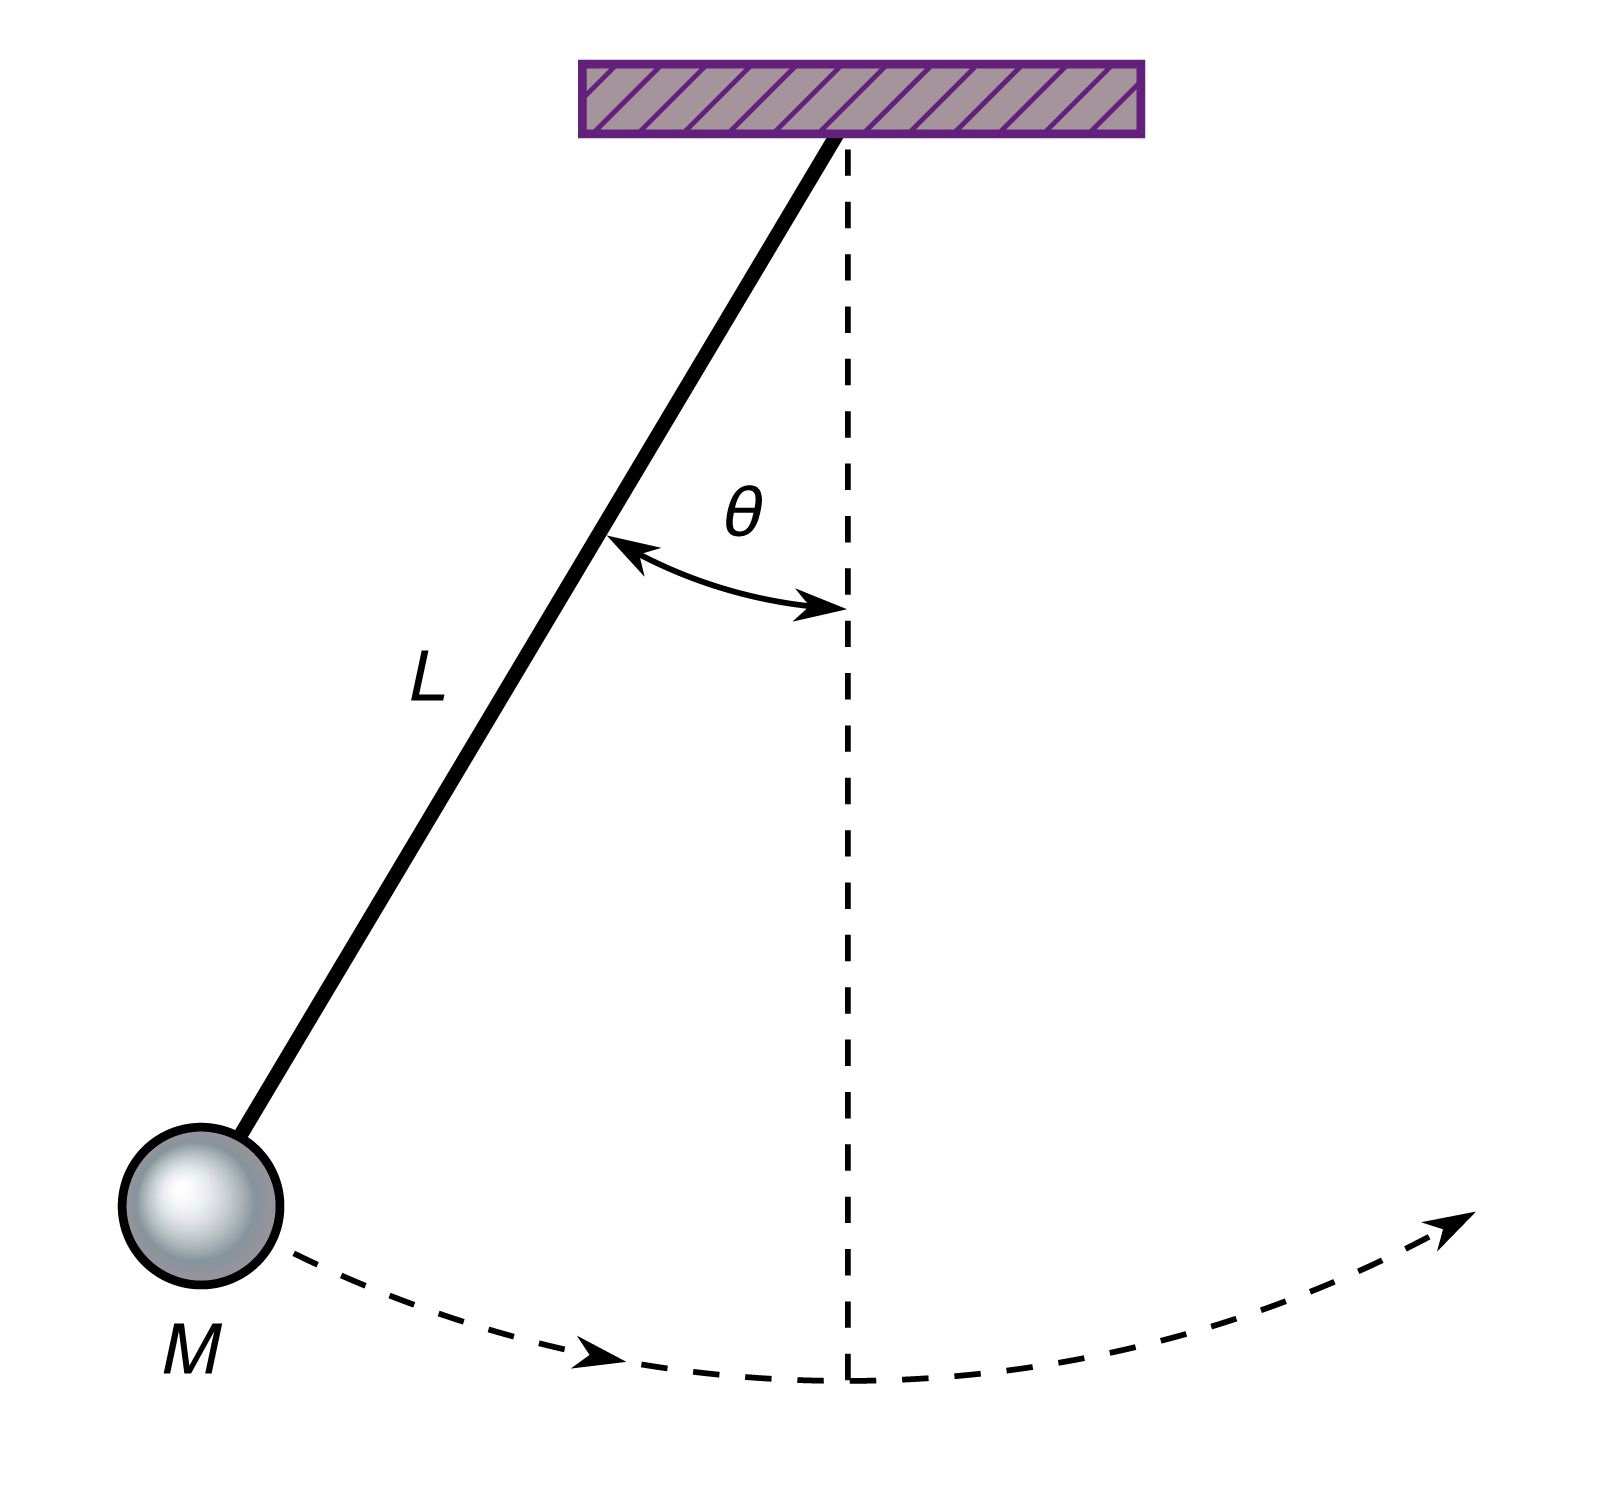
\includegraphics[scale=0.1]{IMG_0200.jpeg}	
		\end{center}
		
		
		
		\vfill
		
		
		
		corso A\\
		Università degli studi di Torino, Torino\\
		4 aprile 2024\\
		
		
	\end{center}
\end{titlepage}
\tableofcontents
\newpage
	
\chapter{Elettrostatica}
\section{Campo elettrostatico}
\definizione{Campo elettrostatico}{
Il campo elettrostatico prodotto in un punto \(P\) da un sistema di cariche ferme è definito come forza elettrostatica risultante \(F\) che agisce su una carica di prova \(q_0\) posta in \(P\) divisa per la carica stessa.
}
In realtà la carica di prova può perturbare la distribuzione di cariche originale, per questo la definizione diventerebbe più precisa se si facesse tendere a zero il valore di \(q_0\). In pratica è sufficiente che \(q_0\) sia molto piccola rispetto alle altre cariche.
\subsection{Dipolo elettrico}
Definiamo \textbf{momento del dipolo}
\[
\vec{p} = q\vec{a}
\]
Consideriamo un punto \(P\) nel quale misuriamo il potenziale, pari alla somma dei contributi delle due cariche:
\[
V(P) = \frac{q}{4\pi \varepsilon_0} \left(\frac{1}{r_1} - \frac{1}{r_2}\right) = \frac{q}{4\pi \varepsilon_0} \left(\frac{r_2 - r_1}{r_1r_2}\right)
\]
Ipotizziamo che \(P\) sia molto distante dal dipolo (rispetto alla distanza \(a\)) così che \(r_1\) e \(r_2\) siano sempre più assimilabili a due segmenti paralleli. Andiamo poi a tracciare un segmento perpendicolare a \(r_1\) fino a \(r_2\) evidenziando la distanza \(r_2 - r_1 \approx a\cos\vartheta\). 

\subsubsection{Potenziale del dipolo}
Con le seguenti approssimazioni andiamo a riscrivere il potenziale:
\[
r_2 - r_1 \approx a\cos\vartheta \qquad \qquad r_1r_2 \approx r^2
\]
\[
V(P) = \frac{q}{4\pi \varepsilon_0} \left(\frac{a\cos\vartheta}{r^2}\right) = \frac{p}{4\pi \varepsilon_0 r^2}
\]
Vediamo come a grandi distanze il potenziale del punto \(P\) dia \textit{informazioni solo sul momento di dipolo} e non sulle due cariche o sulla loro distanza reciproca. A parità di momento si potranno avere due cariche ravvicinate e molto cariche o più distanti e meno cariche.


\subsubsection{Campo elettrico del dipolo}
Riscrivendo \(r\) e \(\cos\vartheta\) esprimiamo il potenziale come
\[
V(P) = \frac{q}{4\pi \varepsilon_0} \left(\frac{a\textcolor{orange}{\cos\vartheta}}{\textcolor{red}{r^2}}\right) 
\]
\[
V(P)= \frac{p}{4\pi\varepsilon_0}\frac{1}{\textcolor{red}{x^2 + y^2 + z^2}}\textcolor{orange}{\frac{z}{\sqrt{x^2 + y^2 + z^2}}} = \frac{p}{4\pi\varepsilon_0}\frac{z}{(x^2+y^2+z^2)^{\frac{3}{2}}}
\]\\

\noindent
Dalla relazione \(\vec{E} = -\vec{\nabla}V\) otteniamo l'espressione del campo elettrico
\[
\vec{E} = \left( \frac{p}{4\pi\varepsilon_0}\frac{3xz}{r^5},\;\ \frac{p}{4\pi\varepsilon_0}\frac{3yz}{r^5},\;\ \frac{p}{4\pi\varepsilon_0}\left(\frac{3z^2}{r^5}-\frac{1}{r^3}\right)\right) 
\]

\[
E(P) = \frac{p}{4\pi\varepsilon_0r^3}\sqrt{3\cos^2\vartheta + 1}
\]
Concludiamo osservando che il campo elettrico del dipolo varia con \(r^3\) (il monopolo con \(r^2\)) e dipende anche dall'angolo \(\vartheta\).


\section{Lavoro elettrico}
Quando su una carica \(q_0\) agisce una forza \(\vec{F}\) \textit{di qualsiasi natura}, possiamo definire sempre un campo elettrico \(\vec{E}\) che chiamiamo \textbf{campo elettromotore}
\[
\vec{E} = \frac{\vec{E}}{q_0} \;\ \to \;\ \vec{F} = q_0 \vec{E}
\]
di cui non conosciamo necessariamente la natura; nel caso di un insieme di cariche ferme questo coinciderà con il campo elettrostatico, ma in questo caso studiamo il caso più generale.

Suddividendo il percorso da \(A\) a \(B\) in segmenti infinitesimi \(d\vec{s}\) calcoliamo il lavoro come integrale di linea del campo \(E\) lungo \(C_1\) 

\[
dW_1 = \vec{F}\cdot d\vec{s} = q_0\vec{E} \cdot d\vec{s}
\]
\[
 W_1 =  q_0 \int_{C_1} \vec{E} \cdot d\vec{s}
\]

\subsection{Tensione elettrica e forza elettromotrice}
\definizione{Tensione elettrica}{
Il rapporto tra il lavoro compiuto dalla forza \(\vec{F}\) nello spostamento da \(A\) a \(B\) lungo il percorso \(C_1\) e la carica 


\begin{equation}
	T(A\to B,C_1) \;\ = \;\ \frac{W_1}{q_0} \;\ =\;\ \int_{C_1}\vec{E}\cdot d\vec{s}
\end{equation}

viene definito \textbf{tensione elettrica}.
}
Se si considera un secondo percorso \(C_2\) si trova in generale un lavoro diverso e quindi un diverso valore della tensione elettrica pur essendo i punti \(A\) e \(B\) gli stessi.


Se studiamo il lavoro lungo un percorso chiuso invece troviamo
\[
W = \oint \vec{F} \cdot d\vec{s} = q_0\oint\vec{E}\cdot d\vec{s}
\]
\definizione{Forza elettromotrice}{
Il rapporto tra lavoro compiuto sulla carica e la carica stessa per il percorso chiuso, ovvero l'integrale di linea circuitazione di campo elettrico
\begin{equation}
\mathcal{E} = \oint\vec{E}\cdot d\vec{s}
\end{equation}
viene definito \textbf{forza elettromotrice} relativa al percorso chiuso \(C\).
}
Sviluppando l'integrale
\begin{align*}
	\oint\vec{F}\cdot d\vec{s} =& \int_{C_1}\vec{F}\cdot d\vec{s} + \int_{-C_2}\vec{F}\cdot d\vec{s} \\
							   =& \int_{C_1}\vec{F}\cdot d\vec{s} - \int_{C_2}\vec{F}\cdot d\vec{s} \\
							   =& W_1 - W_2
\end{align*}
vediamo che in generale per un percorso chiuso il lavoro è diverso da zero. Tuttavia andremo a studiare il comportamento del \textit{campo elettrostatico} che è conservativo e di conseguenza ha circuitazione nulla. 


\subsection{Potenziale elettrostatico ed energia potenziale}
Se il campo è conservativo, non dipendendo dal percorso  seguito l'espressione della tensione elettrica può essere riscritta semplicemente come l'integrale tra \(A\) e \(B\) 
\[
\int_{A}^B\vec{E}\cdot d\vec{s} = f(B) - f(A)
\]
dove \(f\) è una particolare funzione definita a meno di una costante arbitraria e che rinominiamo \(V\) \textbf{potenziale elettrostatico}. 
\definizione{Differenza di potenziale elettrostatico}{
Possiamo definire una \textbf{differenza di potenziale} pari a 
\begin{equation}
\Delta V = - \int_{A}^B\vec{E}\cdot d\vec{s} 
\end{equation}
}
Ricordando che ad ogni forza conservativa è associata una determinata energia potenziale e che il lavoro della forza conservativa è pari all'opposto della variazione della corrispondente energia potenziale
\[
W = -\Delta U_e
\]
\textit{Sono riportate in appendice alcune precisazioni sulle definizioni di potenziale elettrostatico e di energia potenziale (\ref{precisazioni potenziale})}. \\


\noindent
Dalle definizioni precedenti possiamo scrivere le seguenti relazioni
\[
W = q_0 \mathcal{E}  \qquad\qquad \Delta U_e = q_0 \Delta V
\]
\[
W = -q_0 \Delta V \qquad\qquad  \Delta U_e = - q_0 \mathcal{E}
\]

\dimostrazione{: il "campo elettrostatico è conservativo"}{
	Dimostriamo che il campo elettrostatico di una qualsiasi distribuzione di carica è conservativo; cominciamo dal caso più semplice del campo generato da una carica puntiforme:
	\[
	dW = \boldsymbol{q_0}\vec{E} \cdot d\vec{s} = \frac{\boldsymbol{q_0}q}{4\pi\varepsilon_0} \frac{\hat{u}_r \cdot d\vec{s}}{r^2} =  \frac{\boldsymbol{q_0}q}{4\pi\varepsilon_0} \frac{dr}{r^2}
	\]
	Si ottiene che il lavoro da \(A\) a \(B\), caratterizzati dalle distanze \(r_A\) e \(r_B\) dall'origine, vale
	\begin{align*}\label{sviluppo lavoro}
		W =&  \frac{\boldsymbol{q_0}q}{4\pi\varepsilon_0} \int_A^B  \frac{dr}{r^2} \\
		=& -\left(\frac{q_0 q}{4\pi \varepsilon_0 r_B} - \frac{q_0 q}{4\pi \varepsilon_0 r_A}\right)
	\end{align*}
	indipendente dal percorso seguito.
}

\section{Flusso di campo elettrico}
Definiamo flusso di un campo vettoriale \(\vec{E}\) l'integrale
\[
\Phi (\vec{E}) = \int_{\Sigma} \vec{E}\cdot \hat{u}_n \: d\Sigma
\]
dove \(\hat{u}_n\) è il versore normale alla porzione infinitesima di superficie \(d\Sigma\). Vediamo che il prodotto scalare fa sì che contribuisca solo la componente di campo vettoriale ortogonale alla superficie. 

\begin{figure}[h]
	\centering
	\incfig{gauss_subs_1}
\end{figure}

Mostriamo come il flusso \textit{dipenda solo dall'angolo solido sotto il quale la superficie vede la carica}. Prima di tutto qualche osservazione geometrica:

\[
d\vartheta = \frac{ds}{r} \qquad \qquad ds' \cos\alpha = ds \;\ \to \;\ d\vartheta = \frac{ds'\cos\alpha}{r}
\]
\[
d\Omega= \frac{d\Sigma_0}{r^2} \qquad \qquad d\Sigma \cos\alpha = d\Sigma_0 \;\ \to \;\ d\Omega = \frac{d\Sigma\cos\alpha}{r^2}
\]

\begin{figure}[h]
	\centering
	\incfig{gauss_1}
\end{figure}


Andiamo ora a calcolare il flusso attravgausserso \(d\Sigma\):
\begin{align*}
	d\Phi =& \vec{E} \cdot \hat{u}_n d\Sigma \\ 
		  =& \frac{q}{4\pi\varepsilon_0 r^2} \hat{u}_r \cdot \hat{u}_n \: d\Sigma \\
		  =& \frac{q}{4\pi\varepsilon_0 r^2} |\hat{u}_r||\hat{u}_n|\textcolor{red}{\cos\alpha\: d\Sigma} \\ 
		  =& \frac{q}{4\pi\varepsilon_0 r^2} |\hat{u}_r||\hat{u}_n|\textcolor{red}{\: d\Sigma_0} \\
		  =& \frac{q}{4\pi\varepsilon_0  \textcolor{orange}{r^2}} \textcolor{orange}{\: d\Sigma_0} \\
		  =& \frac{q}{4\pi\varepsilon_0}\: \textcolor{orange}{d\Omega} \quad \to \quad \Phi = \frac{q}{4\pi\varepsilon_0}\Omega
\end{align*}
Quindi se consideriamo una superficie chiusa si ha un angolo solido 
\[
d\Omega = \frac{4\pi r^2}{r^2} = 4\pi
\]
e di conseguenza
\begin{equation}
	\verde{\Phi = \frac{q}{\varepsilon_0}}
\end{equation}
Se la carica esterna il flusso è nullo (le cariche esterne contribuiscono solo al campo elettrico). Inoltre se consideriamo più cariche, o addirittura una distribuzione omogenea di cariche si hanno i seguenti valori di flusso:
\[
\text{distribuzione finita di cariche: }\qquad \Phi = \oint \vec{E} \cdot \hat{u}_n \: d\Sigma \;\ = \;\ \sum_i \frac{q_{i(int)}}{\varepsilon_0}
\]
\[
\text{distribuzione continua di cariche: }\qquad \Phi = \frac{1}{\varepsilon_0}\int \rho(x,y,z) \:d\tau 
\]




\subsection{Rotore di un campo vettoriale}
Viene definito rotore del campo elettrico \(\vec{E}\) il prodotto vettoriale
\[
\vec{\nabla} \wedge \vec{E} = \left|\begin{array}{ccc}
	\hat{u}_x & \hat{u}_y & \hat{u}_z \\
	\frac{\partial}{\partial x} & \frac{\partial}{\partial y} & \frac{\partial}{\partial z} \\
	E_x & E_y & E_z 
\end{array}\right| = \left(\frac{\partial E_z}{\partial y}-\frac{\partial E_y}{\partial z}\right)\hat{u}_x + \left(\frac{\partial E_x}{\partial z}-\frac{\partial E_z}{\partial x}\right)\hat{u}_y + \left(\frac{\partial E_y}{\partial x}-\frac{\partial E_x}{\partial y}\right)\hat{u}_z
\]
Questo rappresenta la capacità del campo elettrico di \textit{formare vortici}, ovvero di generare linee di forza che si richiudono su loro stesse.


Poiché anche il rotore del campo elettrico è un campo vettoriale, è possibile definirne un suo flusso:

\[
\Phi(\vec{\nabla} \wedge \vec{E}) =  \int_{\Sigma}\left(\vec{\nabla} \wedge \vec{E}\right)\cdot \hat{u}_n \: d\Sigma
\]

\teorema{}{
\subsubsection{Teorema di Stokes}
La circuitazione è uguale al flusso del rotore:
\[
\oint_\gamma \vec{E}\cdot d\vec{s} = \int_{\Sigma_\gamma}\left(\vec{\nabla} \wedge \vec{E}\right)\cdot \hat{u}_n \: d\Sigma
\]
Qui è espresso nel caso del campo elettrico dove si ha che la circuitazione è nulla qualunque sia la curva \(\gamma\) (a patto che sia chiusa). Allora il flusso del rotore è nullo qualunque sia la superficie ed è possibile solo se il rotore di \(\vec{E}\) è nullo:

\[
\vec{\nabla} \wedge \vec{E} = 0
\]

Dire che il rotore è nullo equivale a dire che il capo elettrico è \textbf{irrotazionale}, ovvero che le sue linee di forza non possono chiudersi su loro stesse; il campo elettrico "non forma vortici".
}

L'annullarsi del rotore non è un fatto sorprendente. Sappiamo infatti che il rotore di un gradiente è sempre nullo e che il campo elettrostatico conservativo può essere scritto come gradiente della funzione scalare del potenziale elettrostatico \(V\):
\[
\vec{\nabla} \wedge \vec{E} = \vec{\nabla} \wedge \left(-\vec{\nabla} V\right)
\]

\subsection{Divergenza di un campo vettoriale}
L'operatore divergenza si applica ad un campo vettoriale e dà origine ad un campo scalare. Il suo significato intrinseco è espresso da 
\[
d\Phi(\vec{E}) = \vec{\nabla}\cdot\vec{E}\,\ d\tau
\]
Prendendo in considerazioni tanti volumetti \(d\tau\) calcoliamo il flusso infinitesimo del campo \(\vec{E}\) attraverso la superficie infinitesima \(d\Sigma\) del volumetto. Estendendo il risultato a tutto il volume \(\tau\) si osserva che i contributi interni al volume si elidono a vicenda e le uniche superfici che contribuiscono al calolo del flusso sono quelle esterne:
\[
\int_\tau d\Phi(\vec{E}) = \int_\tau  \vec{\nabla}\cdot\vec{E}\,\ d\tau = \oint_\Sigma \vec{E}\cdot\hat{u}_n \,\ d\Sigma
\]


\subsection{Discontinuità di carica}

\newpage
\section{Conduttori}
\definizione{Materiale conduttore}{
	Un materiale è detto conduttore se l'elettrizzazione conseguente allo strofinio si diffonde rapidamente andando ad interessare anche zone lontane da quelle in cui è stata prodotta. 
}
I materiali conduttori sono caratterizzati dal fatto che nel loro interno sono verificate particolari condizioni per cui è possibile il moto di alcune cariche (positive e negative in gas ionizzati e soluzioni elettrolitiche e negative nei conduttori solidi) che li costituiscono.

Il moto degli elettroni liberi in un conduttore in equilibrio elettrostatico è completamente disordinato ottenendo perciò una velocità media nulla delle cariche. Si andrà quindi ad assumere che le cariche siano fisse all'interno di un conduttore e che di conseguenza il campo elettrico si annulli:
\[
\vec{E} = 0 \qquad\qquad \text{all'interno}
\]
fatto che comporta le seguenti conseguenze:
\begin{enumerate}
	\item \(\Phi(\vec{E}) = 0\) attraverso qualsiasi superficie gaussiana interna al conduttore. L'annullarsi del flusso implica l'annullarsi della carica. Si ha quindi che l'eccesso di carica su un conduttore può esistere solo in superficie con densità superficiale \(\sigma\);
	\item Avendo definito \(\vec{E} = - \vec{\nabla}V\) si ha che il potenziale è costante in tutto il conduttore:
	\[
	V(P_1) - V(P_2) = \int_{P_1}^{P_2}\vec{E} \cdot d\vec{s} = 0 \quad \implies \quad V(P_1) = V(P_2) = V_0
	\]
	dove \(V_0\) corrisponde al lavoro di estrazione.
	Questo fa sì che la superficie del conduttore sia equipotenziale e, quindi, che il campo elettrico sia localmente ortogonale alla superficie (il gradiente è ortogonale alle curve di livello) e valga
	
	\begin{figure}[H]
		\centering
		\incfig{cilindro_piano}
	\end{figure}
	\[
	\Phi(\vec{E}) = 2 E\Sigma = 2 E\pi R^2 = \frac{q}{\varepsilon_0} = \frac{\sigma 2\pi R^2}{\varepsilon_0} \quad \implies \quad \vec{E} = \frac{\sigma}{\varepsilon_0}\hat{u}_n
	\]
\end{enumerate}

\paragraph*{Campo elettrico indotto}
Avvicinando un conduttore carico o scarico ad un altro corpo carico, ovvero introducendolo in un campo elettro esterno \(\vec{E}_\text{est}\) il campo elettrico interno non sarebbe più nullo; senonché questo fatto provoca un movimento di elettroni che si spostano per l'azione del campo elettrico esterno e si accumulano in una zona della superficie, lasciando sul resto della superficie un eccesso di carica positiva: tra queste zone si crea un campo elettrostatico indotto \(\vec{E}_i\) che contrasta il movimento degli elettroni fino a raggiungere l'equilibrio quando
\[
\vec{E}_i + \vec{E} = 0
	\]
\begin{figure}[H]
	\centering
	\incfig{lastre_piastra}
\end{figure}

\section{Dielettrici}
Consideriamo un condensatore piano carico ed isolato; sulle armature si distribuisce una carica \(q_0\) uniforme distribuita con densità \(\sigma_0\). Tra le armature, poste a distanza \(h\), si genera il campo elettrico \(\vec{E}_0\) e una differenza di potenziale \(V_0\) che valgono
\[
\vec{E}_0 = \frac{\sigma_0}{\varepsilon_0} \qquad\qquad V_0 = \frac{q_0}{C_0} = E_0 h
\]
Introduciamo tra le armature una lastra conduttrice di spessore \(s < h\). Si osserva che la differenza di potenziale tra le armature diminuisce. Ciò accade a causa del campo elettrico indotto che va a generarsi nella lastra conduttrice che va ad annullare il campo \(E_0\) al suo interno. La nuova differenza di potenziale vale
\[
V = E_0h - E_0 s = E_0(h-s) < V_0
\]
\definizione{Materiale isolante}{
Un materiale è detto isolante se l'elettrizzazione conseguente allo strofinio resta localizzata nella zona in cui è stata prodotta. All'interno di un materiale isolante non possono avvenire spostamenti di cariche di alcun tipo: non si osserva la presenza di carica elettrica libera.
}
Se ripetiamo l'esperimento con una lastra di materiale isolante si osserva che \(V\) è minore, a parità di spessore \(s\), di quello misurato con il materiale conduttore. Più precisamente la differenza di potenziale diminuisce linearmente all'aumentare di \(s\) fino a raggiungere un valore minimo \(V_k\) quando \(s\) è massima.

Chiamiamo \textbf{costante dielettrica relativa} il valore, che si osserva essere sempre maggiore di 1,
\[
k_e = \frac{V_0}{V_k} > 1
\] 
\begin{figure}[H]
	\centering
	\incfig{condensatore_dielettrico}
\end{figure}
Vediamo come la capacità del condensatore aumenti se tra le armature è presente un materiale isolante:
\[
C_k = \frac{q_0}{V_k} = \frac{q_0}{V_0/k_e} = k_eC_0
\]
Il campo elettrico \(E_k\) interno al dielettrico vale
\[
E_k = \frac{\boldsymbol{V_k}}{h} = \frac{\boldsymbol{V_0}}{\boldsymbol{k_e}h} = \frac{E_0}{k_e} = \frac{\sigma_0}{k_e\varepsilon_0}
\]
Quindi la variazione di campo elettrico dovuta al materiale isolante vale
\[
E_0 - E_{k} = \frac{\sigma_0}{\varepsilon_0} -  \frac{\sigma_0}{k_e\varepsilon_0} = \frac{k_e - 1}{k_e}\frac{\sigma_0}{\varepsilon_0}
\]
da cui riscrivo \(E_k\) come 
\[
E_k = \frac{\sigma_0}{\varepsilon_0} - \frac{k_e - 1}{k_e}\frac{\sigma_0}{\varepsilon_0}
\]
dove \(\sigma_p =  \frac{k_e - 1}{k_e}\sigma_0\) è la densità di carica che immaginiamo depositata sulle facce della lastra dielettrica con segno opposto a quello della carica libera sull'armatura contigua. Queste cariche sono il risultato dei processi microscopici che avvengono all'interno del dielettrico sotto l'azione del campo elettrico esterno. 

Introduciamo inoltre il concetto di \textbf{suscettività elettrica del dielettrico} \(\chi_e = k_e - 1\) che  misura di quanto questo si polarizza in risposta ad un campo elettrico. \\

\noindent
Nella nuova condizione del condensatore si misurano i seguenti valori:
\[
V_k = \frac{1}{k_e}V_0 \qquad\qquad E_k = \frac{1}{k_e}E_0 \qquad\qquad C_k = k_eC_0
\]
\[
V_k = \frac{1}{\boldsymbol{k_e}}\frac{\sigma_0}{\boldsymbol{\varepsilon_0}}h \qquad\qquad E_k = \frac{1}{\boldsymbol{k_e}}\frac{\sigma_0}{\boldsymbol{\varepsilon_0}} \qquad\qquad C_k = \frac{\boldsymbol{k_e\varepsilon_0}}{h}\frac{q_0}{\sigma_0}
\]\\
chiamiamo \(\varepsilon = k_e\varepsilon_0\) \textbf{costante  dielettrica assoluta del dielettrico}
\[
V_k = \frac{\sigma_0}{\boldsymbol{\varepsilon}}h \qquad\qquad E_k = \frac{\sigma_0}{\boldsymbol{\varepsilon}} \qquad\qquad C_k = \frac{\boldsymbol{\varepsilon}}{h}\frac{q_0}{\sigma_0}
\]
\subsection{Polarizzazione}
Se si applica un campo elettrico ad un materiale dielettrico, essendo gli elettroni legati agli atomi e non distribuiti in una sorta di gas libero di muoversi, avviene soltanto uno spostamento locale delle cariche.


\paragraph*{Polarizzazione per deformazione}
Possiamo dire che gli elettroni siano distribuiti in modo simmetrico rispetto al nucleo dell'atomo dove troviamo anche il centro di massa del sistema. Questo quando è sottoposto ad un campo elettrostatico esterno, il centro di massa subisce uno spostamento. Per effetto del campo elettrico esterno, gli atomi che erano privi di momento di dipolo elettrico assumono un dipolo elettrico pari alla carica del nucleo moltiplicata lo spostamento subito dal nucleo rispetto al centro degli orbitali.

\begin{center}
	\textcolor{red}{atomo}
\end{center}

L'atomo diventa quindi ben descrivibile se pensato come un dipolo; chiamiamo \(\vec{x}\) il vettore che unisce il centro della carica negativa al nucleo e definiamo il momento di dipolo elettrico
\[
\vec{p} = Z e \vec{x}
\]
parallelo e concorde al vettore campo elettrico.

\paragraph*{Polarizzazione per orientamento} 
Esistono sostanze le cui molecole presentano un momento di dipolo intrinseco: si tratta di molecole poliatomiche la cui distribuzione delle cariche è tale che il centro delle cariche negative non coincida quello delle cariche positive. 

L'acqua è una delle molecole con valore molto maggiore della norma. Se non è presente nessun campo elettrico i singoli dipoli sono orientati casualmente per via degli urti dovuti al moto di agitazione termica e il momento totale del sistema macroscopico è nullo.se è presente un campo elettrico esterno, i momenti di dipolo si orientano parzialmente paralleli ad esso e il loro valore medio è quindi diverso da zero.

Andando a considerare ogni momento di dipolo possiamo definirne uno medio concorde con \(\vec{E}\)
\[
\vec{p}_m \,\ < \,\ \vec{p}_0
\]

\begin{figure}[H]
	\centering
	\incfig{polarizzazione}
\end{figure}
 
\paragraph*{Definizione del vettore polarizzazione}
Prendiamo in considerazione un volumetto \(d\tau\) contenente \(dN\) atomi/molecole, il momento di dipolo risultante è dato dal prodotto \(\Delta\vec{p} = \Delta N \vec{p}_m\).  Il vettore intensità di polarizzazione, anche detto vettore di polarizzazione elettrica e indicato con \(\vec{P}\), è il momento di dipolo elettrico per unità di volume posseduto dal materiale. Lo definiamo come
\[
\vec{P} =\frac{\Delta \vec{p}}{\Delta\tau} = \frac{\Delta N}{\Delta \tau}\vec{p}_m
\]
più precisamente come il limite per \(\tau \to 0\)
\[
\vec{P} = \lim_{\Delta\tau\to 0}\frac{\Delta \vec{p}}{\Delta\tau} = \lim_{\Delta\tau\to 0}\frac{\Delta N}{\Delta \tau}\vec{p}_m
\]

che chiamiamo \textbf{vettore di polarizzazione} e dove \(n\) è il numero atomi/molecole per unità di volume. 
\definizione{Polarizzazione elettrica (Wikipedia)}{
La polarizzazione elettrica, in fisica, descrive la \textit{formazione di dipoli elettrici} all'interno di un materiale, costituiti dalla carica elettrica posseduta dagli atomi e dalle molecole di cui esso è composto, in seguito all'applicazione di un campo elettrico. La polarizzazione elettrica si manifesta in particolare nei materiali dielettrici, e genera la presenza di un campo elettrico aggiuntivo all'interno di essi.}


La maggior parte dei dielettrici sono \textbf{lineari isotropi} e in essi risulta che \(\vec{P}\) è proporzionale al campo \(\vec{E}\):
\[
\vec{P} = \varepsilon_0(k_e -1)\vec{E} = \varepsilon_0 \chi_e \vec{E}
\]
Esistono mezzi anisotropi come i cristalli nei quali la suscettività elettrica \(\chi_e\) non è un numero ma bensì un tensore. Il parallelismo tra \(\vec{P}\) ed \(\vec{E}\) è mantenuto solo su alcune direzioni che coincidono con gli assi cristallografici.

\subsubsection{Campo elettrostatico prodotto da un dielettrico polarizzato}
Consideriamo il condensatore piano carico con all'interno una lastra di dielettrico polarizzato uniformemente, abbiamo quindi un vettore polarizzazione \(\vec{P}\) uguale in tutti i punti della lastra. Suddividiamo la lastra in tanti volumetti \(d\tau = d\Sigma_0 dh\). Come abbiamo visto prima il vettore polarizzazione vale
\[
\vec{P} = \frac{d\vec{p}}{d\tau}
\]
ovvero momento di dipolo complessivo per unità di volume.

Sulle facce del prisma si vanno a depositare una serie di cariche \(\pm q_p\) con densità \(\pm \sigma_p\) dando un momento di dipolo al prisma.

\paragraph{Polarizzazione uniforme}
Per trovare il campo elettrico andremo a studiare quello generato dai tanti dipoli che formano il dielettrico attraverso l'espressione del momento di dipolo complessivo del prisma
\[
d\vec{p} = \vec{P}d\tau = P \,\ d\Sigma_0 d\vec{h}
\]

\begin{figure}[H]
	\centering
	\incfig{cubi}
\end{figure}

Sostituiamo al prisma un sistema costituito da cariche \(\pm dq_p\) distribuite con densità \(\pm\sigma_p\). Sapendo che 
\[
\vec{p} = q \vec{h} \quad \to \quad q = \frac{\vec{p}}{\vec{h}} \quad \implies \quad \boldsymbol{dq_p =} \frac{d\vec{p}}{d\vec{h}} \boldsymbol{= Pd\Sigma}
\]
notiamo quindi che la densità di carica vale quanto il modulo del vettore polarizzazione:
\[
\boldsymbol{\pm\sigma_p =} \pm\frac{dq_p}{d\Sigma} \boldsymbol{=\pm P}
\]
Se sovrapponiamo due volumetti di questo tipo si osserva che la carica sulla faccia in comune si annulla. Perciò la lastra di dielettrico è equivalente a due distribuzioni di carica \(\pm \sigma_p = \pm P\).

Se generalizziamo il risultato per un dielettrico non simmetrico si hanno le seguenti espressioni 
\[
\boxed{\sigma_p = \vec{P} \cdot \hat{u}_n \qquad \qquad dq_p = \vec{P} \cdot \hat{u}_n \,\ d\Sigma}
\]

Se la polarizzazione è uniforme non si manifestano cariche all'interno del dielettrico, ma solo sulla superficie. Come abbiamo visto il processo che genera \(\pm \sigma_p\) fa sì che la somma delle cariche sia nulla:
\[
\oint dq_p =  \vec{P} \cdot \hat{u}_n \,\ d\Sigma = 0
\]

\paragraph{Polarizzazione non uniforme}
Prendiamo in considerazione una polarizzazione non uniforme lungo l'asse \(x\)  ed esaminiamo il valore della carica sulla faccia comune \(d\Sigma = dy \,\ dz \) dei due prismi.

\begin{figure}[H]
	\centering
	\incfig{parall}
\end{figure}

\[
dq_p = \vec{P} \cdot \hat{u}_x d\Sigma = P_x dydz
\]
\[
-dq'_p = \vec{P}'\cdot \hat{u}'_x d\Sigma = -P'_x dydz
\]
Studiamo la differenza
\[
dq_p -dq'_p = \boldsymbol{(P_x - P'_x)}dydz = \boldsymbol{-\frac{\partial P}{\partial x} dx} dy dz = -\frac{\partial P}{\partial x}d\tau
\]
Se estendiamo il risultato a tutte le dimensioni otteniamo 
\[
dq_p = \left(-\frac{\partial P_x}{\partial x}-\frac{\partial P_x}{\partial y}-\frac{\partial P_z}{\partial z}\right)d\tau = -\left(\vec{\nabla}\cdot\vec{P}\right)d\tau
\]
distribuita con densità \(\rho_p\) pari a meno la divergenza di \(\vec{P}\)
\[
\rho_p = \frac{dq_p}{d\tau} = -\vec{\nabla}\cdot\vec{P}
\]
In un dielettrico in cui la polarizzazione non è uniforme, oltre alla densità superficiale di carica di polarizzazione esiste una densità di carica di polarizzazione uguale in ogni punti all'opposto della divergenza del vettore polarizzazione \(\vec{P}\).

Vediamo come, poiché la carica totale di polarizzazione deve essere nulla, ritroviamo il teorema della divergenza: esprimiamo la carica totale come somma di carica di polarizzazione di superficie e di volume
\[
\oint_\Sigma \sigma_p \, d\Sigma + \int_\tau \rho_p \, d\tau = 0
\]
dalle espressioni ottenute in precedenza di \(\sigma_p\) e da quella appena ottenuta di \(\rho_p\) 
\[
\sigma_p = \vec{P}\cdot\hat{u}_n \qquad \qquad \rho_p = - \vec{\nabla}\cdot\vec{P}
\]
riscriviamo gli integrali come
\[
\oint_\Sigma \vec{P}\cdot\hat{u}_n \, d\Sigma  - \int_\tau \vec{\nabla}\cdot\vec{P} \, d\tau = 0 \quad \to \quad \oint_\Sigma \vec{P}\cdot\hat{u}_n \, d\Sigma  = \int_\tau \vec{\nabla}\cdot\vec{P} \, d\tau
\]

\subsubsection{Calcolo di \(V\) e di \(\vec{E}\) conoscento \(\vec{P}\)}

\subsection{Induzione dielettrica}
Definiamo il vettore induzione elettrica
\[
\vec{D} = \varepsilon_0\vec{E} + \vec{P	}
\]
Per osservare perché questo è definito in questo modo studiamo l'espressione del flusso di campo elettrico in presenza di cariche di polarizzazione:
\[
\oint_{\Sigma} \vec{E} \cdot \hat{u}_n \,\ d\Sigma = \frac{q + q_p}{\varepsilon_0}
\]
dal teorema della divergenza sappiamo che 
\[
\oint_{\Sigma}\vec{E} \cdot \hat{u}_n \,\ d\Sigma = \int_{\tau} \vec{\nabla}\cdot \vec{E} \,\ d\tau
\]
quindi possiamo scrivere
\[
\int_{\tau} \vec{\nabla}\cdot \vec{E} \,\ d\tau = \frac{q + q_p}{\varepsilon_0} \quad \to \quad \vec{\nabla}\cdot \vec{E} \int_{\tau}  d\tau = \frac{q + q_p}{\varepsilon_0} \quad \to \quad \vec{\nabla}\cdot \vec{E} = \frac{1}{\tau}  \frac{q + q_p}{\varepsilon_0}
\]
\begin{center}
	\textcolor{red}{Assumendo che la divergenza sia costante penso si ricavi così. guarda p.79 Mazzoldi}
\end{center}
da cui
\[
\vec{\nabla}\cdot \vec{E} = \frac{\rho + \rho_p}{\varepsilon_0}
\]
Ricordando che la densità volumica delle cariche polarizzate \(\rho_p\) è uguale a meno la divergenza del vettore polarizzazione: \(\rho_p = - \vec{\nabla}\cdot \vec{P}\), possiamo riscrivere la divergenza di campo elettrico come

\[
\vec{\nabla}\cdot \vec{E} = \frac{\rho - \vec{\nabla}\cdot \vec{P}}{\varepsilon_0}  \quad \to \quad \varepsilon_0\vec{\nabla}\cdot \vec{E} = \rho - \vec{\nabla}\cdot \vec{P} \quad \to \quad \vec{\nabla} \cdot \left(\varepsilon_0\vec{E} + \vec{P}\right) = \rho
\]
da cui otteniamo che \(\vec{D} = \varepsilon_0\vec{E} + \vec{P}\) è il vettore la cui divergenza è uguale alla densità volumica delle cariche libere:
\[
\vec{\nabla} \cdot \vec{D} = \rho
\] 	

\subsubsection{Il flusso di \(\vec{D}\) dipende solo dalle cariche libere}
Sia \(\Sigma\) una superficie chiusa che contenga una carica libera \(q_0\) e una parte del dielettrico polarizzato. 

Calcoliamo il flusso di campo elettrico attraverso la superficie \(\Sigma\) come somma dei contributi di
\begin{center}
	 Carica libera \(q_0\) \hspace{0.2cm} Carica di polarizzazione di superficie (\(\sigma_p\)) \hspace{0.2cm} Carica di polarizzazione di volume (\(\rho_p\))
\end{center}

\begin{figure}[H]
	\centering
	\incfig{gauss_vettore_D}
\end{figure}	
\[
\Phi(\vec{E}) = \frac{q_0}{\varepsilon_0} + \frac{\int_{\Sigma_1} \sigma_p \,\ d\Sigma}{\varepsilon_0} + \frac{\int_\tau \rho_p \,\ d\tau}{\varepsilon_0}
\]
sapendo che 
\[
\sigma_p = \vec{P}\cdot\hat{u}_n \qquad \qquad \rho_p = - \vec{\nabla}\cdot\vec{P}
\]
riscriviamo il flusso come 
\[
\Phi(\vec{E}) = \frac{q_0}{\varepsilon_0} + \frac{\int_{\Sigma_1} \vec{P}\cdot\hat{u}_n \,\ d\Sigma}{\varepsilon_0} - \frac{\int_\tau  \vec{\nabla}\cdot\vec{P} \,\ d\tau}{\varepsilon_0}
\]
dal teorema della divergenza sappiamo che 
\[
\int_\tau  \vec{\nabla}\cdot\vec{P} \,\ d\tau = \oint_{\Sigma_1 + \Sigma_2} \vec{P}\cdot\hat{u}_n \,\ d\Sigma
\]
quindi riscriviamo il flusso come 
\begin{align*}
	\Phi(\vec{E}) =& \frac{q_0}{\varepsilon_0} + \frac{\int_{\Sigma_1} \vec{P}\cdot\hat{u}_n \,\ d\Sigma}{\varepsilon_0} - \frac{ \oint_{\Sigma_1 + \Sigma_2} \vec{P}\cdot\hat{u}_n \,\ d\Sigma}{\varepsilon_0} \\
				  =& \frac{q_0}{\varepsilon_0} + \frac{\int_{\Sigma_1} \vec{P}\cdot\hat{u}_n \,\ d\Sigma}{\varepsilon_0} - \frac{ \int_{\Sigma_1} \vec{P}\cdot\hat{u}_n \,\ d\Sigma}{\varepsilon_0} - \frac{ \int_{\Sigma_2} \vec{P}\cdot\hat{u}_n \,\ d\Sigma}{\varepsilon_0} \\
				  =& \frac{q_0}{\varepsilon_0} - \frac{1}{\varepsilon_0} \int_{\Sigma_2} \vec{P}\cdot\hat{u}_n \,\ d\Sigma
\end{align*}
Il flusso del campo elettrostatico \(\vec{E}\) attraverso \(\Sigma\) contiene un contributo non nullo dovuto alla carica di polarizzazione. Poiché nella parte esterna al dielettrico si annulla il vettore polarizzazione \(\vec{P} = 0\), calcolare il flusso attraverso \(\Sigma_2\)

Poiché \(\vec{P}\) è nullo fuori dal dielettrico, il flusso di \(\vec{P}\) "investe" solamente la superficie \(\Sigma_2\); per questo motivo calcolarlo su tutta \(\Sigma\) o solamente su \(\Sigma_2\) è indifferente:
\[
\int_{\Sigma_2}\vec{P}\cdot\hat{u}_n \,\ d\Sigma = \oint_{\Sigma}\vec{P}\cdot\hat{u}_n \,\ d\Sigma
\]
Ora dalla definizione di \(\vec{D}\)
\[
\vec{D} = \varepsilon_0 \vec{E} + \vec{P}
\]
definiamo il flusso di \(\vec{D}\) attraverso \(\Sigma\) come
\begin{align*}
	\oint_\Sigma \left(\varepsilon_0 \vec{E} + \vec{P}\right)\cdot\hat{u}_n \,\ d\Sigma =& \oint_\Sigma \varepsilon_0 \vec{E}\cdot\hat{u}_n \,\ d\Sigma +  \oint_\Sigma\vec{P}\cdot\hat{u}_n \,\ d\Sigma  \\
	=& \varepsilon_0 \Phi(\vec{E}) +  \oint_\Sigma\vec{P}\cdot\hat{u}_n \,\ d\Sigma
\end{align*}
Sapendo che
\[
\Phi(\vec{E}) = \frac{q_0}{\varepsilon_0} - \frac{1}{\varepsilon_0} \int_{\Sigma_2} \vec{P}\cdot\hat{u}_n \,\ d\Sigma \qquad \qquad   \oint_{\Sigma}\vec{P}\cdot\hat{u}_n \,\ d\Sigma = \int_{\Sigma_2}\vec{P}\cdot\hat{u}_n \,\ d\Sigma 
\]
riscriviamo il flusso di \(\vec{D}\) come 
\begin{align*}
	\oint_\Sigma \left(\varepsilon_0 \vec{E} + \vec{P}\right)\cdot\hat{u}_n \,\ d\Sigma =& \varepsilon_0\left(\frac{q_0}{\varepsilon_0} - \frac{1}{\varepsilon_0} \int_{\Sigma_2} \vec{P}\cdot\hat{u}_n \,\ d\Sigma\right) + \int_{\Sigma_2}\vec{P}\cdot\hat{u}_n \,\ d\Sigma \\
	=& q_0 - \int_{\Sigma_2} \vec{P}\cdot\hat{u}_n \,\ d\Sigma+ \int_{\Sigma_2}\vec{P}\cdot\hat{u}_n \,\ d\Sigma \\
	=& q_0
\end{align*}
Quindi in generale detto \(q\) l'insieme delle cariche libere possiamo scrivere
\[
\oint_\Sigma \vec{D}\cdot\hat{u}_n \,\ d\Sigma = q
\]

\subsection{Dielettrici isotropi e anisotropi}

\subsection{Dielettrici cavi}

\subsection{Energia elettrostatica nei dielettrici}

\subsection{Meccanismi di polarizzazione nei dielettrici}

\newpage
\esempio{espressione come condensatori in serie}{
Quando andiamo ad inserire un dielettrico in un condensatore possiamo esprimere la capacità di quest'ultimo come la capacità equivalente di due condensatori, uno vuoto e l'altro riempito dal dielettrico.

Partiamo con questi valori considerando il condensatore vuoto
\[
E_0 = \frac{\sigma_0}{\varepsilon_0} \qquad \qquad V_0 = E_0 h = \frac{\sigma_0 h}{\varepsilon_0} \qquad \qquad D = \varepsilon_0 E_0 = \sigma_0
\]
Inserendo il dielettrico troviamo il campo in esso \(\vec{E}_k\) e un nuovo potenzale \(V_k\):
\[
E_k = kE_0
\]
\[
P = \varepsilon_0(k-1)\boldsymbol{E_k} = \varepsilon_0 \frac{k-1}{\boldsymbol{k}}\boldsymbol{E_0} = \frac{k-1}{k}D = \frac{k-1}{k}\sigma_0
\]
definiamo ora la differenza di potenziale \(V\)
\begin{align*}
	\boldsymbol{V= }\int_{0}^{h-s}\vec{E}_0\cdot d\vec{h} + \int_{0}^{s}\vec{E}_k\cdot d\vec{s} =& E_0(h-s) + E_ks \\
	 =& \frac{\sigma_0}{\varepsilon_0}(h-s) + \frac{\sigma_0}{k\varepsilon_0}s \;\  = \;\ \frac{\sigma_0 h}{\varepsilon_0} \left(\frac{h-s}{h} + \frac{s}{hk}\right)\\
	 =& \frac{\sigma_0 h}{\varepsilon_0} \left(\frac{k(h-s) + s}{hk} \right) \;\ = \;\ \frac{\sigma_0 h}{\varepsilon_0} \left(\frac{hk - sk +s}{hk} \right) \\
	 =& \frac{\sigma_0 h}{\varepsilon_0} \left(1 + s\frac{1-k}{hk} \right) \;\ \boldsymbol{=} \;\ \boldsymbol{V_0\left(1 - \frac{k-1}{k}\frac{s}{h} \right)} \\
\end{align*}
La differenza di potenziale diminuisce linearmente con \(s\) ed è minima quando il dielettroc riempie completamente lo spazio tra le armature (\(s = h\)). In tal caso infatti il campo vale ovunque \(E = E_0/k\) e la differenza di potenzile, integrale di linea da \(0\) a \(h\) varrebbe \(V = E_0h/k = V_0/k\).

Se andiamo a riscrivere il potenziale come
\[
V = \frac{\boldsymbol{\sigma_0}}{\varepsilon_0}\frac{\boldsymbol{\Sigma}}{\Sigma}\left(h - \frac{k-1}{k}s\right) = \frac{\boldsymbol{q}}{\varepsilon_0\Sigma}\left(h-\frac{k-1}{k}s\right)
\]
}
dividendo per \(q\) carica libera sulle armature del condensatore si trova
\[
\frac{V}{q} = \frac{h-s}{\varepsilon_0 \Sigma} + \frac{s}{\varepsilon_0 k \Sigma}
\]
\[
\frac{1}{C} = \frac{1}{C_0} + \frac{1}{C_k}
\]
La capacità equivalente del condensatore parzialmente riempito di dielettrico è uguale a quella di due condensatori in serie, uno vuoto e uno pieno di dielettrico.

\chapter{Appendice}
\section{Precisazioni sulle definizioni di potenziale elettrostatico ed energia potenziale}\label{precisazioni potenziale}
Dallo sviluppo del lavoro della forza elettrostatica otteniamo
\[
W = -\left(\frac{q_0 q}{4\pi \varepsilon_0 r_B} - \frac{q_0 q}{4\pi \varepsilon_0 r_A}\right)
\]\\
Sapendo che
\[
W = -q_0 \Delta V = -\Delta U 
\]\\
possiamo definire le differenze di potenziale e di energia potenziale come
\[
V(B) - V(A) = \left(\frac{ q}{4\pi \varepsilon_0 r_B} - \frac{q}{4\pi \varepsilon_0 r_A}\right)
\]
\[
U_e(B) - U_e(A) = \left(\frac{q_0 q}{4\pi \varepsilon_0 r_B} - \frac{q_0q}{4\pi \varepsilon_0 r_A}\right)
\]\\
Ricordando che sia il potenziale sia l'energia potenziale son definiti a meno di una costante additiva possiamo considerare le variazione delle funzioni
\[
V(r) = \frac{q}{4\pi\varepsilon_0 r} + C_V\qquad \qquad U_e(r) = \frac{q_0q}{4\pi\varepsilon_0 r} + C_{U_e}
\]\\
Possiamo determinare completamente \(V(r)\) e \(U_e(r)\) imponendo che  entrambi si annullino per \(r\to\infty\):
\[
r\to \infty \qquad V(\infty) = 0 \qquad U_e(\infty) = 0 \qquad \implies \;\ C_V = C_{U_e} = 0
\]\\
In conclusione abbiamo le seguenti definizioni di potenziale elettrostatico generato da una carica puntiforme \(q\) a distanza \(r\) e di energia potenziale di \(q_0\) nel campo di \(q\):
\[
V(r) = \int_{r}^{\infty} \vec{E}\cdot d\vec{s} = \frac{q}{4\pi\varepsilon_0 r}
\]
\[
U_e(r) \;\ = \;\ q_0V(r) \;\ = \;\ q_0\int_{r}^{\infty} \vec{E}\cdot d\vec{s} = \frac{q_0q}{4\pi\varepsilon_0 r}
\]

\end{document}